\documentclass{article} %specifies the document being created is an article
\usepackage{graphicx} %tells LaTeX we want to include images in the document 
\graphicspath{ {./images/} } %this points to your image folder, replace images with the name of the folder you are using to store the images displayed in this document. (Note: This folder must be in the same folder where your LaTeX document is saved)
\usepackage[acronym,automake]{glossaries}

\makeglossaries

\usepackage{natbib} % this allows you work on the references and citations in Harvard format
\pagestyle{empty}

\newacronym{rdbms}{RDBMS}{Relational Database Management System}
\newacronym{uml}{UML}{Unified Modeling Language}
\newacronym{ccci}{CCCI}{Complexity, Conformity, Changeability and Invisibility}
\newacronym{erd}{ERD}{Entity Relationship Diagram}
\usepackage{pdfpages}

\begin{document} %start the document
	
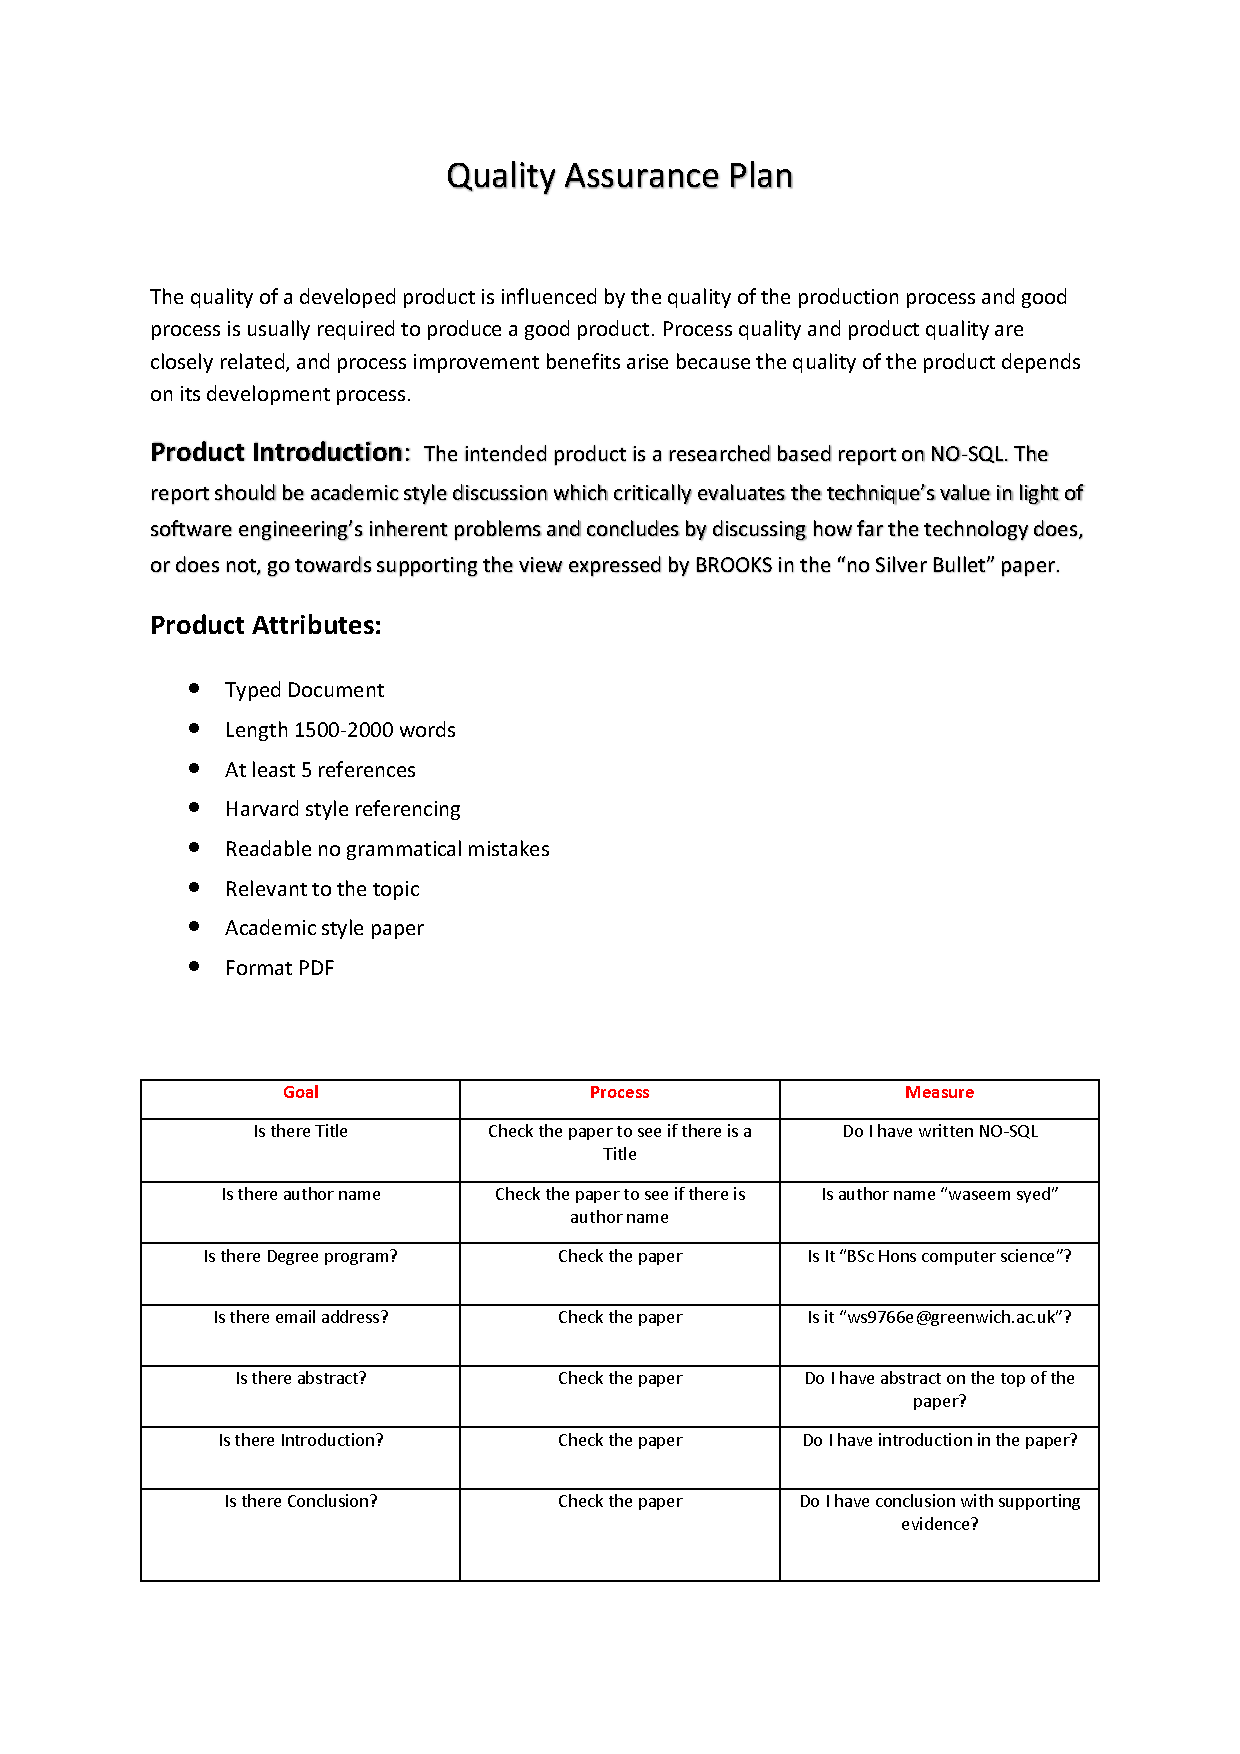
\includepdf[pages=-]{qac.pdf}


\title{NO-SQL} %title of document
\author{Waseem Syed - BSc Hons Computer Science \\
			ws9766e@greenwich.ac.uk} %author of document (i.e. you)

\maketitle %prints the title on the page



{
	\centering


} %this command can be used to center any text within LaTeX.




\section{Abstract}
Brooks (1987) illustrates that there are four components that make software engineering 
hard and these are  complexity, conformity, changeability and invisibility (CCCI). 
He says, “Building software will always be hard. There is inherently no silver bullet.” (Brooks, 1987).  
Brooks outlined these four problems in software engineering about  30 years ago and this 
paper aims to find out if, since then, NO-SQL is a silver bullet. The discussion in this paper will be 
investigating what NO-SQL is doing to tackle \gls{ccci}, features
of No-SQL databases and look to see how they affect the problems, whether positively or negatively.

\section{Introduction}
No-SQL database stands for "Not Only SQL" or "Not SQL." 
No-SQL databases arose in response to those limitations of SQL. No-SQL systems store and manage data in 
ways that allow for high operational speed and great flexibility on the part of the developers. 
No-SQL is a non-relational database management system, that does not require a fixed schema, avoids joins, and is easy to scale. No-SQL database is used for distributed data stores with humongous data storage needs. 
Many were developed by companies like Google, Amazon, Yahoo, and Facebook that sought better ways to store content or process data for massive websites. Unlike SQL databases, many No-SQL databases can be scaled horizontally across hundreds or thousands of servers. 

\cite{tang2016performance} says that nowadays there are more than 225 No-SQL databases
according to the real-time statistics and different
No-SQL databases have different implementation mechanisms,
storage characteristics, configurations and optimization
methods, which brings more challenges in No-SQL selection. In
this paper we try to test No-SQL performance to give
suggestion to anyone who need to select No-SQL in different
application scenarios.\\

There can be a lot of small entities in a software system which adds to the complexity of its nature. 
In big software systems, there are inherently many entities, therefore the system is very complex. This paper will make an investigation into No-SQL to see 
whether complexity reduces.   Software systems also need to conform to specification 
and laws. This means that the specification of the system needs to be understood and know exactly what 
the end user requires otherwise the system is a failure because there could be requirements that are 
not implemented. 
The need for systems to change is huge in the modern world. Changeability
is partly down to failing systems but also due to consumer/customer demand. Consider a mobile application.
If that mobile application has a bug, a software engineer can update the application to remove the
bug without the customer/consumer having to return a physical item. Software systems, in terms of 
the coding and design, is invisible. 


When it comes to building a wardrobe, one can follow a 
process by viewing diagrams. These diagrams relate to physical things such as nails and screws.
This makes it easier for the person building the wardrobe to visualise how it all comes together.
When it comes to software, there are \acrshort{uml} diagrams to help one visualise a system. 
When working on large system, these diagrams are complex, need to conform, need to change to
meet new requirements and are invisible.  


\section{Discussion} %sections within LaTeX can be created like this
\subsection{Complexity}

\cite{lombardo2012issues} explains the problems faced by using a No-SQL as the main
data storage. Most importantly how to flatten a complex data model
and how to manage the execution of complex queries.
A No-SQL DB is mainly organized in uncorrelated tables.
Thus, a complex and intrinsically relational data model has
to be flattened and partitioned in various No-SQL tables.
Two different partitioning policies are possible, vertical
partitioning, where each column of a high level relational
table is stored into a separate No-SQL table and horizontal
partitioning, where different tuples are stored in 
No-SQL tables.To manipulate and retrieve data,
database administrators are given a primitive set of
commands. Complex business functionality requires
significant amount of design and programming to
implement, although simpler business models may
be able to suffice with the primitive command set
supplied.\\
In software projects, the reduction of complexity may
be aided by use of No-SQL depending on
the functionality required from the database itself. No-SQL database is schema free, which 
means that we don't to define the fields of a table in advance. \\
\cite{tang2016performance} divide No-SQL into four categories: key-value, document store,
column family store and graph database. He did experiments on databases and he concluded that all databases have their limitations, some are good in loading and executing workloads but some don't have good average performance.\\
\cite{burtica2012practical} says that Google has demonstrated, a shared-nothing system scales faster, 
because adding new nodes will not create bottlenecks or slow down the system.
This system also increases the availability of the system, since there is no
single point of failure. This model is called sharding.\\
\cite{mohamed2014relational} explains that complexity in relational databases is higher and 
No-SQL databases have the capabilities to store unstructured, semi structured or structured data.
It seems trade between 
complexity lays within the system, rather than how
much complexity there is. It is important to consider
what is functionality is required from the database
when choosing a database system, in order to reduce
the complexity which the developers will face.

\subsection{Changeability}

Changeability is an expected behaviour of a software and successful 
software adapt to its any change.
\citealp{chandra2015base} explains the characteristics of No-SQL and one of 
them is Schema-less, like Key-value stores, so new values can be added at runtime
without affecting any other data stored.\\
\cite{hecht2011nosql} says that due to very simple data structure, key value stores are completely
schema free. New values of any kind can be added at runtime
without influencing system availability.
No-SQL databases allow insertion of data without having predefined a
schema for the database to adhere to.  This complements agile methodologies in
software projects well. It allows focus on the design
and adapting to changes in the software, rather than
the schema which supports the data.
In SQL making any changes require
a change in the schema, requires the schemas
to be modified first and for the database to be
migrated to the new schema. This may require
a migration project in order to complete schema
changes. Database schema migration can involve
writing change scripts which need to be written from
scratch for each change and this fits in poorly with the ideals of
agile methodology, including the aim to meet rapidly
changing requirements.\\
No-SQL's dynamic schema supports frequency and
speed of change in a positive way. Changes in
databases can be done quickly, scaling well with
the size of the change to be made while having
the capability to avoid down-times with the service
and without the need of any scripts or migration
projects. The changes can be made simply and
effectively. This helps to reduce the effect of
problems encountered due to the required and
expected changeability in software.


\subsection{Conformity}
In software engineering all software systems must conform to laws and 
processes, different standards and formats. There are other systems and environments in 
place such as externalised APIs, which the system needs to conform to. 
As we know that Databases are created with the goal of storing data,
it is important for such technologies to conform to the Data Protection Act, which
specifies a multitude of factors to ensure data security.
No-SQL's enhanced ability to adapt to changes means that it is more suitable to conforming
to sets of changing standards or requirements compared to \acrshort{rdbms}.

\subsection{Invisibility}


Unlike \acrshort{rdbms}, in No-SQL we don't make Entity Relationship Diagrams
so visualisation of a No-SQL database model is difficult because it lacks
explicit schema. On the other hand \acrshort{rdbms} make use of \acrshort{erd} to diagrammatically
represent its schema. \acrshort{uml} Class Diagrams have been proposed and used
as a way of constructing representations of No-SQL
schemas. \cite{delfosse2012uml} has suggested how to map
a graph store database to \acrshort{uml} Class Diagrams but it does not 
tackle the problem of possible inconsistency throughout the database.
It can be said that \acrshort{rdbms} is superior in this aspect.
The strict and rigid schema provides a useful way of
representing the data storage model. Opposing this
to No-SQL which inconsistent, making
it difficult to meaningfully convey the model in a
diagrammatic format.



\section{Conclusions}

No-SQL databases are becoming a major part of the database landscape today, and with their many advantages, they can be a real game changer in the enterprise arena. Lower cost, easier scalability, and open source features make No-SQL an appealing option for many companies looking to integrate in Big Data. However, No-SQL is still a relatively young technology without the set of standards that SQL databases like MySQL offer.  As with any major business decision, IT leaders need to weigh their options and determine what features are most important to them in a database. Some suggest that No-SQL is the way of the future. It is obvious that four inherent problems of software engineering not
completely solved with introduction of No-SQL. We can notice that dynamic
nature of No-SQL favours changeability, but it comes on cost of
its invisibility. In terms of \acrshort{ccci}, No-SQL reduced complexity compared 
to complexity of \acrshort{rdbms}. No-SQL does not support strong encryption and security
features. Invisibility is still 
an issue and always will be because software is not something to can touch. 
Invisibility increases as complexity rises.
it's enhanced ability to adapt to changes means that it is more suitable to conforming to sets of changing standards or requirements compared to \acrshort{rdbms}. One should consider the requirements of the system when decide which database to use.  At the end of the day, the choice between No-SQL and SQL depends on the complex business needs of an organization and volume and variety of data it consumes
No-SQL as a technology by itself, does not serve to
be a "silver bullet" which Brooks Jr. proposed and
does not appear capable of becoming one in the near
future, due to its schema-less nature. A single No-SQL database 
does not tackle \acrshort{ccci} but a Hybrid Database system of MySQL and No-SQL 
can be used as suggested by \cite{8528120}.



\section{Evaluation}

No-SQL does make progress to finding the silver bullet for software engineering, but it is clear the four components are always found together when trying to 
tackle an individual component. For example,  when complexity increases then invisibility increases too. 
This is just one example of how they are all linked together. As there are positives 
and negatives for No-SQL, it cannot be a silver bullet because there are negatives. 
\cite{hecht2011nosql} suggests that "Use the right tool for the job" is  the slogan of
 No-SQL, because every No-SQL database is
specialized on certain use-cases.
First of all, we have to evaluate their data in order to
identify a suitable data model to avoid unnecessary complexity
due to transformation or mapping tasks. Queries which should
be supported by the database have to be considered at the same
time, because these requirements massively influence the
design of the data model. Since there isn't any common query language
available, every store differs in its supported query feature set.
Then we have to trade between high
performance through partitioning and load balanced replica
servers, high availability supported by asynchronous
replication and strict consistency. Beside these
different requirements, also durability mechanism, community
support and useful features like versioning influence the
database selection. In general, key value stores should be used
for very fast and simple operations, document stores offer a
flexible data model with great query possibilities, column
family stores are suitable for very large datasets which have to
be scaled at large size, and graph databases should be used in
domains, where entities are as important as the relationships
between them. So we can deduce that No-SQL are not Brooks
"Silver Bullet".
A silver bullet would “cure” software engineering from all negatives of \acrshort{ccci}. 


\section{Future Work}

For future work on this subject, there could be an investigation into schemas
and a redesign of the databases will be required, meeting both
the advantages provided by No-SQL and \acrshort{rdbms} databases.








\bibliographystyle{agsm}
\bibliography{BIBLIOGRAPHY} %import biblography to be used for references here, replace the bibliography.bib with the name of your .bib file
\clearpage

\section{Appendices}


\printglossary[type=\acronymtype,title=Acronyms]




\end{document} %end the document